\documentclass{article}

\usepackage{blindtext}
\usepackage{graphicx}
\usepackage{wrapfig}
\usepackage[skip=1ex]{caption}
\usepackage{subcaption}
\usepackage{mdframed}
\usepackage{amsmath}
\usepackage{amsfonts}
\usepackage{amssymb}
\usepackage{amstext}
\usepackage{cancel}
\usepackage{enumitem}
\usepackage[english]{babel}
\usepackage{helvet}
\usepackage{microtype}
\usepackage[pdftex]{hyperref}
\usepackage{float}
\usepackage{nicematrix}
\usepackage{xcolor}
\usepackage{tikz}
\usepackage{geometry}
\geometry{
    a4paper,
    left=2cm,
    right=2cm,
    top=1cm,
    bottom=1cm
}

\special{papersize=8.5in,11in}
\setlength{\pdfpageheight}{\paperheight}
\setlength{\pdfpagewidth}{\paperwidth}

% Macros

% Make inline frac bigger
\newcommand\ifrac[2]{{\displaystyle\frac{#1}{#2}}}

% Aliases
\def\wstar{\overset{*}{\rightharpoonup}}
\def\grad{\nabla}
\def\lap{\Delta}
\def\nt{\notag}
\def\dt{\partial_t}
\def\hal{\ifrac{1}{2}}
\def\ep{\varepsilon}
\def\cK{\mathcal{K}}
\def\cA{\mathcal{A}}
\def\cS{\mathcal{S}}
\def\cV{\mathcal{V}}
\def\Q{\mathbb{Q}}
\def\R{\mathbb{R}}
\def\R{\mathbb{R}}
\def\C{\mathbb{C}}

% Custom operators
\DeclareMathOperator{\Err}{Err}






\begin{document}



\title{Written Assignment 3}

\author{Niraj Venkat}

\date{}

\maketitle

\vspace{.8cm}
\boxed{\text{Exercise} \quad 1}\\\\


An \emph{analytic} function has infinitely many derivatives in its domain. For our proof, we only need a function to be
twice-differentiable.\\
We state Liouville's theorem:
\begin{mdframed}
    Suppose $f$ is analytic in the open set that contains a ball $B_r(z_0)$ of radius $r$ centered at $z_0$,
    and that $|f(z)| \le c$ holds on $\partial B_r(z_0)$ for some constant $c$. Then for all $k \ge 0$ we have: $$|f^{(k)}(z_0)| \le \frac{k!\,c}{r^k}$$
\end{mdframed}
Simply put: if $f$ is bounded, $f$ must be constant.\\
This holds for \emph{harmonic} functions as well, 
in particular our function $\phi : M \rightarrow \R$ where $k=2$
and $\lap \phi = 0$.\\\\


\vspace{1.8cm}
\boxed{\text{Exercise} \quad 2}\\\\


This admits different proofs:
\begin{itemize}
    \item
        Suppose we had a function $f$ such that $\lap f = \lap \phi = c$. Then by linearity of the Laplacian we have:
        $$
            \lap (\phi - f) = \lap (f - \phi) = 0
        $$
        Liouville's Theorem says that both functions $\phi - f$ and $f - \phi$ must be constant.\\
        $c=0$ is the only value that satisfies this condition.

    \item
        Stokes' theorem (divergence theorem) says the following:
        \begin{mdframed}
            For any vector field, we 
            can relate the divergence of the vector field within the volume $V$ 
            to the outward flux of the vector field through the surface $S = \partial V$.
        \end{mdframed}
        In our case, we apply this theorem to the vector field which is the gradient $\grad \phi$.\\
        The Laplacian $(\lap = \grad \cdot \grad)$ is the divergence of gradient,
        so for some compact domain $M$ without boundary $(\partial M = \emptyset)$ we have:
        \begin{align*}
            \int_M \grad \cdot \grad \phi \,dV &= \int_{\partial M} \grad \phi \cdot \hat{n} \,dS = 0\\
            \implies 0 &= \int_M \lap \phi \,dV = \int_M c \,dV = c \,\text{vol}(M)
        \end{align*}
        Because $M$ has some non-negative volume, $c$ cannot be an arbitrary constant. $c$ has to be zero.
\end{itemize}


\pagebreak
\boxed{\text{Exercise} \quad 3}\\\\


% We use the proof of the generalized Stokes Theorem over $k$-dimensional manifolds.
% \href{https://math.uchicago.edu/~may/REU2012/REUPapers/Presman.pdf}{Theorem 5.1 in this writeup by Rick Presman.}\\


According to Stokes' theorem:

\begin{align*}
\int_\partial g \star df &= \int d(g \star df) \\
    &= \int dg \wedge \star df + \int g \wedge d \star df \\
    &= \int dg \wedge \star df + \int g \wedge \star  \lap f \\
    &= \langle \grad g, \grad f \rangle + \langle g, \lap f \rangle
\end{align*}


On the other hand:

\begin{align*}
\int_\partial g \star df &= \langle g, N \cdot \grad f \rangle_\partial
\end{align*}


This proves Green's first identity:

\begin{align*}
\langle \lap f, g \rangle &= -\langle \grad f, \grad g \rangle + \langle N \cdot \grad f, g \rangle_\partial
\end{align*}


\vspace{1.8cm}
\boxed{\text{Exercise} \quad 4}\\\\


If there is no boundary:

\begin{align*}
    \langle g, N \cdot \nabla f \rangle_\partial = 0
\end{align*}

If $f = g$, then Green's first identity becomes:
\begin{align*}
    \langle \lap f,f\rangle &= -\langle \nabla f, \nabla f\rangle + 0\\
        &= -||\grad f||^2 \le 0
\end{align*}

This means the operator $\lap$ is negative semidefinite, and $-\lap$ is positive semidefinite (PSD).\\
The set of PSD matrices is convex, as such many tools in numerical linear algebra (eg: semidefinite 
programming) can be used to find the minimum of the quadratic functions they describe (eg: quadratic forms
$\vec{x}^T A \vec{x}$).


\vspace{1.8cm}
\boxed{\text{Exercise} \quad 5}\\\\

Using figure on the next page as a reference:

\begin{align*}
    w &= b_1 + b_2\\
    h &= |\overline{ip}|\\
    \cot\alpha &= \frac{b_1}{h}\\
    \cot\beta &= \frac{b_2}{h}\\
    \frac{w}{h} &= \cot\alpha + \cot\beta
\end{align*}
    

\pagebreak
\boxed{\text{Exercise} \quad 6}\\\\

\begin{wrapfigure}{r}{0.3\textwidth}
    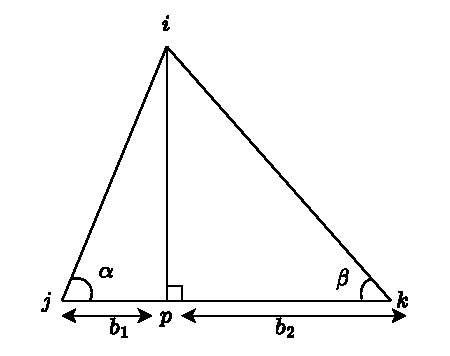
\includegraphics[scale=0.8]{figs/tri.pdf}
\end{wrapfigure}

Triangle $ijk$ has base $b = |e| = b_1 + b_2$ and height $h$.

Let $e$ be the edge vector for the base edge $jk$, with $i$ as the opposite vertex.\\

The interpolating hat functions $\phi$ are similar to their smooth counterpart, the Dirac delta $\delta$.
It is equal to one at their associated vertex and zero at all other vertices. We associate $\phi$ with vertex $i$.\\

We can expand the interpolating hat function $\phi$ in a Taylor series expansion about the point $x_0$. Since 
the hat function is linear, all higher order terms go to zero.\\
$$
    \phi(x) = \phi(x_0) + \grad \phi \cdot (x - x_0)
$$

Plugging our vertices into this expression:
\begin{align}
    \phi(i) &= 1 \\
    \phi(j) &= \phi(i) + \grad \phi \cdot (j - i) = 0 \\
    \phi(k) &= \phi(i) + \grad \phi \cdot (k - i) = 0
\end{align}

Subtracting (3) - (2):
\begin{align*}
    \phi(k) - \phi(j) &= \grad \phi \cdot (k - i) - \grad \phi \cdot (j - i)\\
        &= \grad \phi \cdot (k - j) = 0
\end{align*}

We get that direction of $\grad \phi$ is perpendicular to $e$. Next we calculate the magnitude of $\grad \phi$
by substituting (1) into (2):
\begin{align*}
    0 &= \phi(i) + \grad \phi \cdot (j - i) = 0 \\
        &= 1 + \grad \phi \cdot (j - i) \\
    1 &=  \grad \phi \cdot (i - j) \\
        &= |\grad \phi| |i - j| \cos(\pi - \alpha) \\
        &= |\grad \phi| \, h \\
    |\grad \phi| &= \frac{1}{h} = \frac{b}{bh} = \frac{|e|}{2A}
\end{align*}

We call $e^\perp$ the vector perpendicular to $e$ with magnitude $|e|$. This gives our desired gradient:
$$
    \grad \phi = \frac{e^\perp}{2A}
$$


\vspace{1.8cm}
\boxed{\text{Exercise} \quad 7}\\\\


Using our previous result $\grad \phi = \ifrac{e^\perp}{2A}$:

\begin{align*}
    \langle \grad \phi, \grad \phi \rangle &= \frac{e^\perp \cdot e^\perp}{4A} \\
        &= \frac{b^2}{4bh} \\
        &= \hal \frac{b}{2h} \\
        &= \hal (\cot\alpha + \cot\beta)
\end{align*}


\vspace{1.8cm}
\boxed{\text{Exercise} \quad 8}\\\\


We consider vertices $i$ and $j$ with opposite edge vectors making angle $\theta$ (labelled $\beta$ in our figure).\\
The opposite edge vectors as labelled in our figure are $e_i = \overline{jk}$ and $e_j = \overline{ki}$

\begin{align*}
    \langle \grad \phi_i, \grad \phi_j \rangle &= \frac{e^\perp_i \cdot e^\perp_j}{4A} \\
    e^\perp_i \cdot e^\perp_j &= |e_i| |e_j| \cos(\pi - \theta) = -|e_i| |e_j| \cos\theta \\
    A &= \hal (e_j \times -e_i) = \hal (e_i \times e_j) = \hal |e_i| |e_j| \sin(\pi - \theta) = \hal |e_i| |e_j| \sin\theta \\
\end{align*}

Altogether:
$$
    \langle \grad \phi_i, \grad \phi_j \rangle = -\hal \cot\theta
$$


\vspace{1.8cm}
\boxed{\text{Exercise} \quad 9}\\\\

In our diagram, primal mesh elements are solid, dual are dashed.\\

Since each dual edge connects the centers of two circles with the corresponding primal edge as a common chord,
each dual edge is a perpendicular bisector of the primal edge.

\begin{wrapfigure}{r}{0.5\textwidth}
    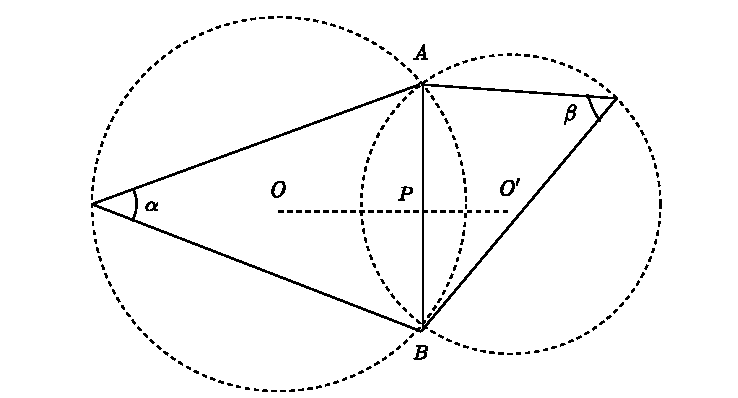
\includegraphics[scale=0.8]{figs/chord.pdf}
\end{wrapfigure}

This can easily be proven:
\begin{itemize}
    \item Let the two circumcircles have circumcentres $O$ and $O^\prime$ where $AB$ is the common chord,
    with intersection point $P$.
    \item $OA=OB$ and $O^\prime A = O^\prime B$ (radii of same circle) So,
    $\triangle OAO^\prime$ and $\triangle OBO^\prime$ are congruent. 
    \item With this we can prove $AP=BP$ and $\angle APO = \angle BPO = \ifrac{\pi}{2}$.
    \item $\therefore OO^\prime$ is the perpendicular bisector of $AB$.
\end{itemize}

Using inscribed angle theorem, we get:\\\\
$\alpha = \hal \angle AOB$ and $\beta = \hal \angle AO^\prime B$.\\

Using angle bisector theorem, we get:\\\\
$\angle AOO^\prime = \hal \angle AOB = \alpha$ and $\angle BO^\prime O = \hal \angle BO^\prime A = \beta$.\\

From the previous result relating the ratio $w/h$ to sum of cotangents we have:
\begin{align*}
    \frac{OO^\prime}{AP} &= \frac{OO^\prime}{AB/2} \\
    \frac{OO^\prime}{AB} &= \hal (\cot\alpha + \cot\beta) \\
    \implies \frac{|e^*_{ij}|}{|e_{ij}|} &= \hal (\cot\alpha + \cot\beta)
\end{align*}























































































































\end{document}
